\documentclass[11pt,a4paper]{article}

\usepackage[left=2cm,text={17cm,24cm},top=3cm]{geometry}
\usepackage[czech]{babel}
\usepackage[utf8]{inputenc}
\usepackage[T1]{fontenc}

\usepackage{url}
\usepackage{tikz}
\usepackage{float}
\usepackage{xcolor}
\usepackage{siunitx}
\usepackage{amsmath}
\usepackage{accents}
\usepackage{comment}
\usepackage{listings}
\usepackage{csquotes}
\usepackage{hyperref}
\usepackage{textcomp}
\usepackage{amsfonts}
\usepackage{breakurl}
\usepackage{etoolbox}
\usepackage{graphicx}
\usepackage{multicol}
\usepackage{multirow}
\usepackage{indentfirst}
\usepackage{supertabular}
\usepackage[titles]{tocloft}
\usepackage{dirtytalk}

\def\UrlBreaks{\do\/\do-} % URL breaking characters

\newcommand{\red}[1]{\textcolor{red}{#1}} % \red{text in red}
\newcommand{\blue}[1]{\textcolor{blue}{#1}} % \blue{text in blue}
\newcommand{\TODO}{\textbf{\textcolor{red}{TODO}}} % red bold TODO
\newcommand{\tilda}{\raisebox{0.5ex}{\texttildelow}} % command \tilda for '~' character

\renewcommand{\cftdot}{}

\setlength\parindent{0pt} % do NOT indent
\graphicspath{{img/}} % path to images

\patchcmd{\thebibliography}{\section*{\refname}}{}{}{}



\makeatletter
\newcommand\xleftrightarrow[2][]{%
  \ext@arrow 9999{\longleftrightarrowfill@}{#1}{#2}}
\newcommand\longleftrightarrowfill@{%
  \arrowfill@\Leftarrow=\Rightarrow}
\makeatother

\begin{document}

\begin{titlepage}

    \begin{center}
        % FIX: lines must end with '%', if not then it will result in an incorrect centering
        \vfill {%
            \Huge{%
                \textsc{%
                    Fakulta informačních technologií\\[3mm]%
                    Vysoké učení technické v~Brně%
                }%
            }%
        }%

        \hfill\\[15mm]

        \begin{figure}[!h]
            \centering
            
\includegraphics[scale=0.3]{vutbr-fit-logo.eps}
        \end{figure}

        \hfill\\[10mm]

        \Huge{
            \textbf{
                TIN
            }
        }

        \hfill\\[-10mm]

        \huge{
            \textbf{
                Teoretická informatika
            }
        }

        \hfill\\[10mm]

        \LARGE{
            \textbf{
                1. domácí úloha
            }
        }
        \vfill

    \end{center}

        \Large{
            Attila Lakatos (xlakat01)\hfill \today
        }

\end{titlepage}

\setlength{\parskip}{0pt}
    \hypersetup{hidelinks}\tableofcontents
\setlength{\parskip}{0pt}

\newpage

\section{1. úloha}
\subsection{a)}

Operácia $\circ$ je definovaná následovne:
\begin{equation}
L_1 \circ L_2 = L_1 \cup \overline{L_2}.
\end{equation}


Musíme dokázať, že následujúci vzťah je platný:
\begin{equation}
L_1, L_2 \in \mathcal{L}_3 \Rightarrow L_1 \cup \overline{L_2} \in \mathcal{L}_3
\end{equation}

Z Věty 3.2(študijná opora - strana 50.) vyplýva, že trieda regularných jazykov je uzavretá vzhľadom k operáciam sjednocenie a komplementu \cite{AA}. Na základe toho môžeme povedať, že

\begin{equation}
L_1, L_2 \in \mathcal{L}_3 \Rightarrow L_1 \circ L_2 \in \mathcal{L}_3
\end{equation}

je platný vzťah.










\subsection{b)}

Najprv si musíme vyjádriť sjednocení množín vzťahom pomocou doplňku a prieniku a to preto, aby sme mohli využiť \textbf{Vetu 4.27} zo Študijného textu. Z tohto dôvodu budeme používať De Morganove pravidlá. Upravíme si
výraz $L_1 \circ L_2$ nasledujúcim spôsobom:

\begin{equation}
L_1 \circ L_2 = L_1 \cup \overline{L_2} = \overline{\overline{L_1 \cup \overline{L_2}}} = \overline{\overline{L_1} \cap \overline{\overline{L_2}}} = \overline{\overline{L_1} \cap L_2}
\end{equation}


Z \textbf{Věty 3.23} vyplýva, že trieda regularných jazykov ze uzavretá voči komplementu, ďalej z \textbf{Věty 4.27} vyplýva, že deterministické bezkontextové jazyky sú uzavreté voči prieniku s regularnými jazykami a doplňku \cite{AA}.


Podľa vyššie uvedených vzťahov môžeme vyhlásiť, že $\overline{\overline{L_1} \cap L_2} \in \mathcal{L}_2$ , teda vzťah je \textbf{platný}.










\subsection{c)}

Budeme predpokladať, že
\begin{equation}
L_1 \in \mathcal{L}_3, L_2 \in \mathcal{L}_2 \Rightarrow L_1 \circ L_2 \in \mathcal{L}_2
\end{equation}
je pravdivý vzťah. $L_1$ a $L_2$ sú dva jazyky nad abecedou $\Sigma$. Vieme, že $L_1 \in \mathcal{L}_3$(regulárny jazyk), môžeme si vyjádriť $L_1$, ako $L_1 = \Sigma^*$ a potom musí platiť:

\begin{equation}
\Sigma^* \cup \overline{L_2} \in \mathcal{L}_2 \Rightarrow \overline{L_2} \in \mathcal{L}_2 \hspace{1cm}\textbf{SPOR}
\end{equation}

Dostali sme sa k \textbf{sporu}, pretože z \textbf{Vety 4.23} vyplýva, že bezkontextové jazyky nie sú uzavreté vzhľadom k operácii doplňok \cite{AA}. Takže vzťah

\begin{equation}
L_1 \in \mathcal{L}_3, L_2 \in \mathcal{L}_2 \Rightarrow L_1 \circ L_2 \in \mathcal{L}_2
\end{equation}
je \textbf{neplatný}.

\newpage
\section{2. úloha}

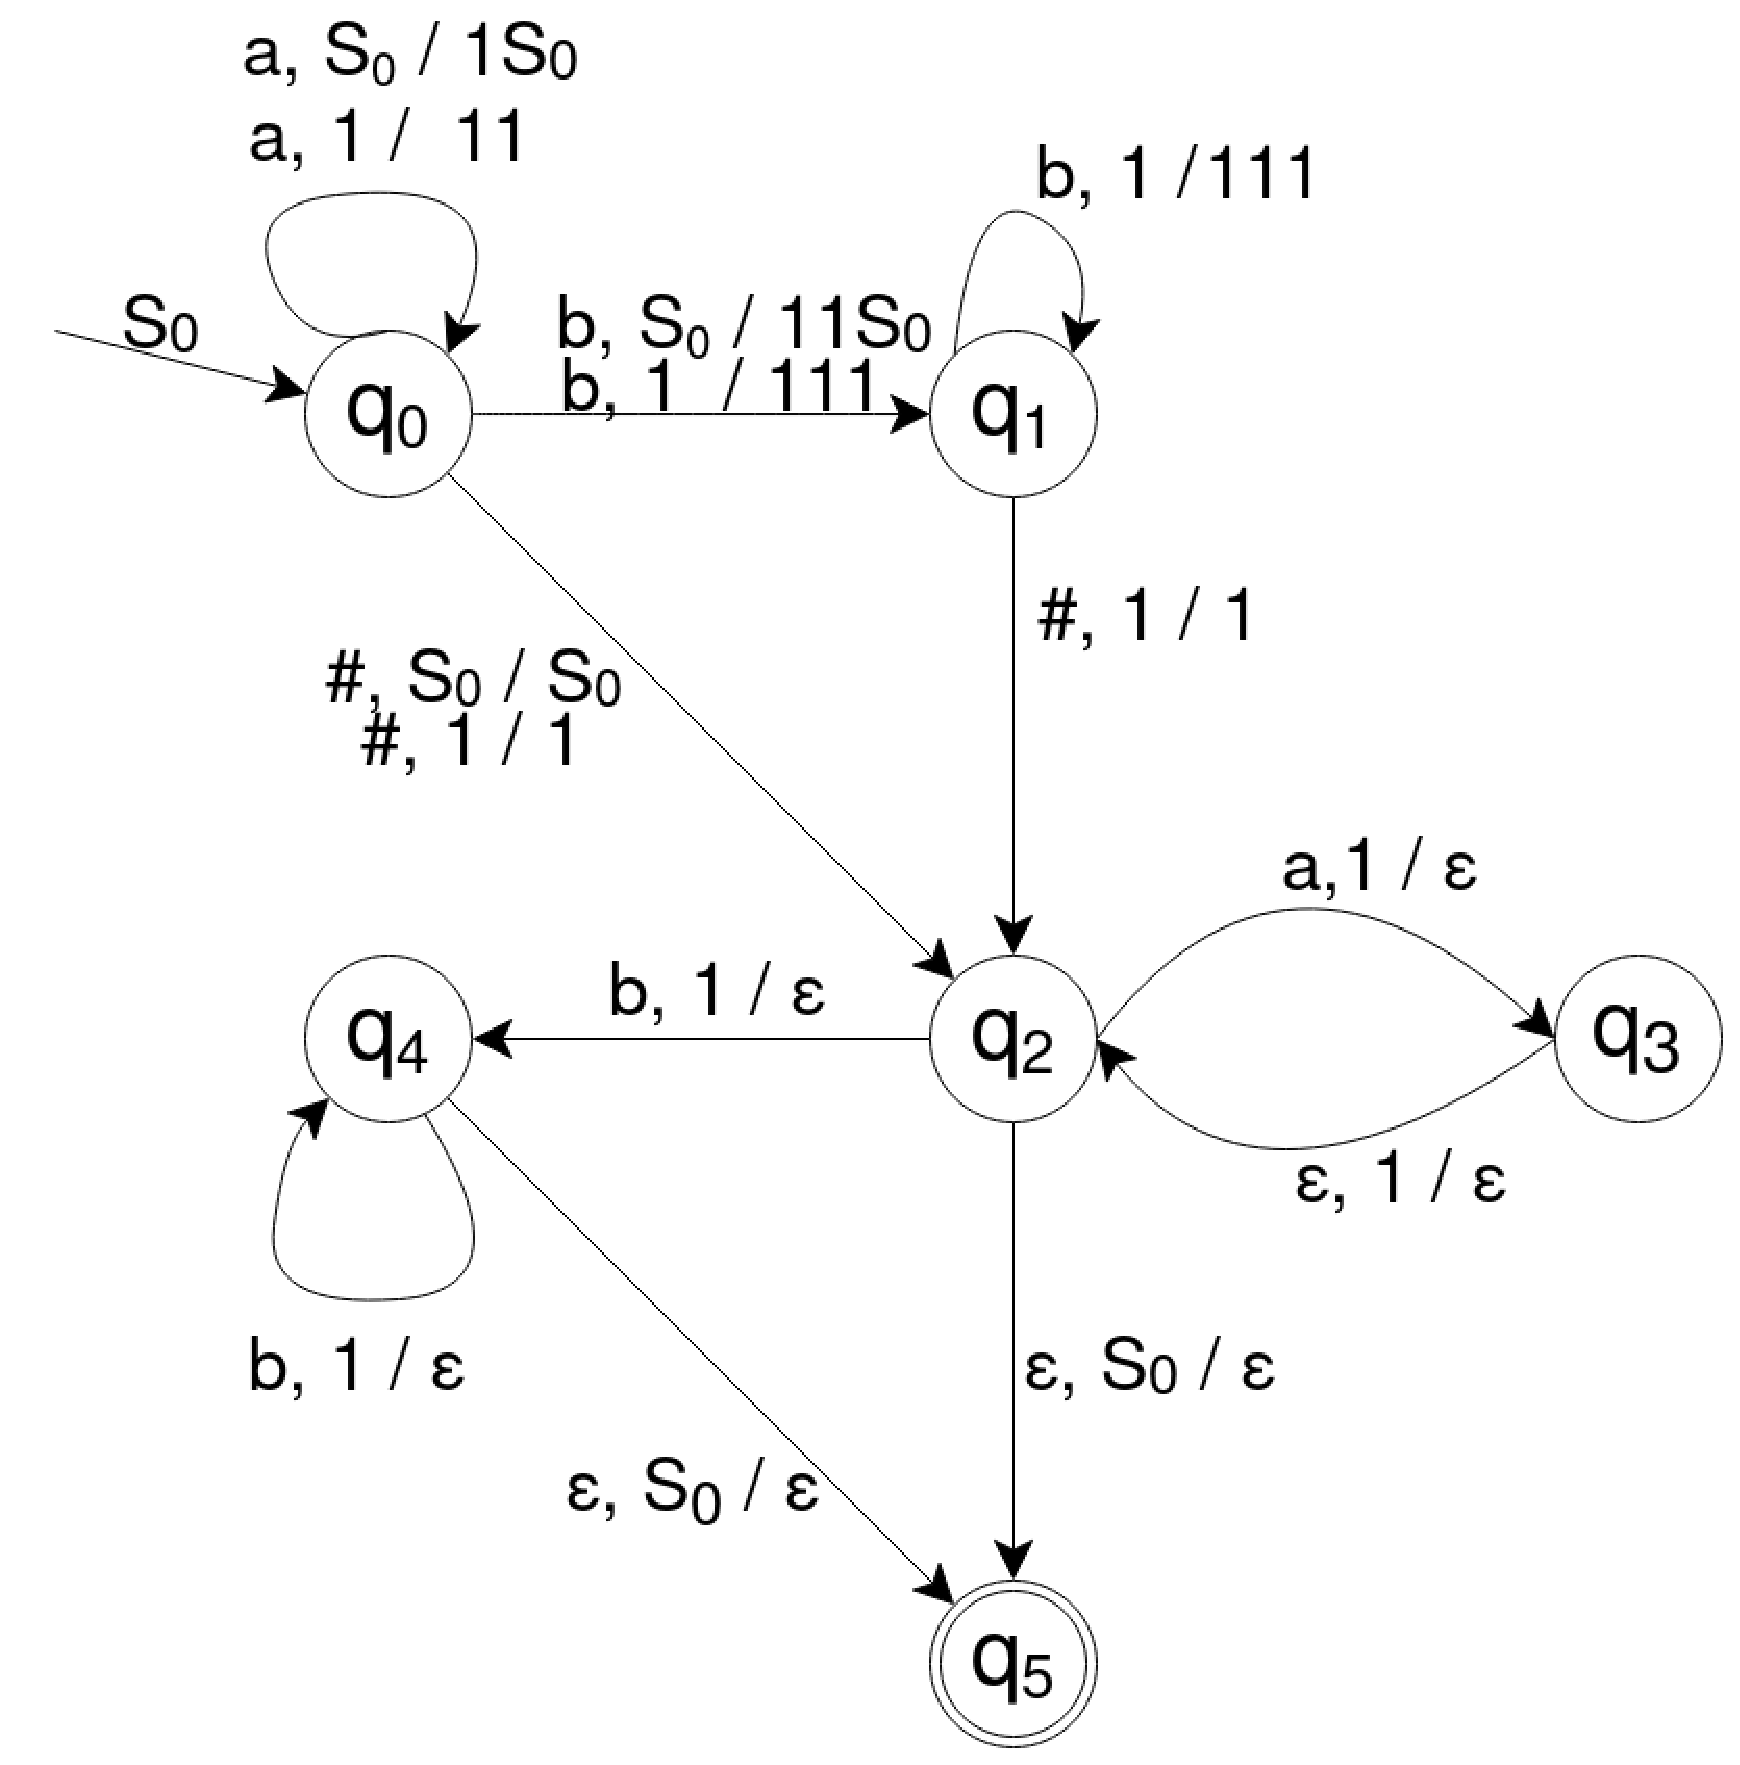
\includegraphics[width=\textwidth]{QFSMpng.eps}

blablabla









\newpage
\section{3. úloha}

Jazyk $L$ z predczádzajúceho príkladu:

\begin{equation}
L = \{a^i b^j \# a^k b^l \hspace{0.17cm}|\hspace{0.17cm} i + 2j = 2k + l\}
\end{equation}

Zaujíma nás vlastnosť, či jazyk spadá do danej triedy jazykov, je užitočné používať tzv. \textit{Pumping lemmu}.
Podľa \textbf{Vety 3.18}: Nechť $L$ je nekonečný regulárny jazyk. Pak existuje celočíselná konstanta \hspace{1cm}p > 0 taková, že platí \cite{AA}:
\begin{equation}
w \in L \land  |w| \ge p \Rightarrow w = x y z \land y \ne \varepsilon \land |xy| \le p \land x y^i z \in L \hspace{0.2cm} pro\hspace{0.2cm} i \ge 0.
\end{equation}

\paragraph{Dôkaz sporom}\mbox{}\\

Budeme predpokládať, že jazyk $L$ je regularný, tak potom podľa \textbf{Vety 3.18} $\exists p > 0$ taková, že platí:

$\forall w \in L : w = a^p \# b^p$ pre ktoré platí $|w| \ge p$ a to platí pretože $2p + 1 \ge p$ a z podmienky $|xy| \le p$ môže nastať len jeden prípad:

\begin{align*}
    \left.
    \begin{array}{r@{}l}
        x = a^j \\
        y = a^k \\
        z = a^{p-j-k} \# b^p
    \end{array}
    \right\rbrace
    \begin{array}{r@{}l}
        j \in \mathbb{N} \land j \ge 0, \\
        k \in \mathbb{N} \land k > 0, \\
        j + k \le p
    \end{array}
\end{align*}

potom náš reťezec $w = x y^i z = a^j a^{k^i} a^{p-j-k} \# b^p = a^{j + k*i + p -j -k} \# b^p = a^{p + i*k - k} \# b^p$ musí patriť do $L$ pre všetky  $i \ge 0$.
Avšak toto \textbf{neplatí}, pretože $p + i*k -k \ne p$ pre všetky $i \ge 0$ (Podmienka môže byť splňena len pre $i = 1$).

$a^{p + i*k - k} \# b^p \notin L$ pre všetky $i \ge 0$. Z toho vyplýva, že jazyk $L$ \textbf{neni regularný}.





\newpage
\section{4. úloha}

\subsection{a)}

Algoritmus, ktorý pre daný nedeterministický konečný automat $A = (Q, \Sigma, \delta, q_0 , F)$ rozhodne, či \hspace{0.3cm} $\forall w \in L(A) : |w| \ge 5$.
\vspace{1cm}

\textbf{Vstup: }\\[-1.8em]
\begin{center}
\begin{minipage}{0.85\textwidth}
    \begin{tabular}{rlcl}
        Nedeterministický konečný automat $A = (Q, \Sigma, \delta, q_0 , F)$
    \end{tabular}
\end{minipage}
\end{center}


\textbf{Výstup}\\[-1.8em]
\begin{center}
\begin{minipage}{0.85\textwidth}
    \begin{tabular}{r|lcl}
        \textit{$\forall w \in L(A) : |w| \ge 5$ }  & \textit{Áno}\\
        \textit{Jinak}  & \textit{Nie}\\
    \end{tabular}
\end{minipage}
\end{center}

\paragraph{Metóda}\mbox{{}}\\

$\textbf{X} \gets \{ \exists w \in \Sigma^* \hspace{0.2cm} \forall i \in \mathbb{N} \land 0 \le i < 5 \hspace{0.2cm} | \hspace{0.2cm} (q_o, w) \vdash^i (q_f, \varepsilon) \land q_f \in F \}$

\textbf{if} $(|X| == 0)$

\hspace{0.55cm} return Áno

\textbf{else}

\hspace{0.55cm} return Nie


\paragraph{Popis metody slovne}\mbox{{}}\\
Na začiatku si vytvoríme množinu, ktorá bude obsahovať všetky reťezce ktoré sú prijímané nedeterministickým konečným automatom $A$ a zároveň délka každého reťezca je menšie ako 5.
Následne kontrolujeme, či počet retezcov v tejto množine sa rovná nule. Ak áno, tak platí, že $\forall w \in L(A) : |w| \ge 5$, vrátime Áno, inak Nie.

\subsection{b)}

\paragraph{Demonštrácia}\mbox{{}}\\
\begin{enumerate}
  \item Najprv si vytvoríme množinu $X$, ktorá bude obsahovať všetky reťezce, ktoré majú délku menšiu ako 5.

  \item Hovoríme, že vstupný retezec $w$ je prijímán nedeterministickým konečným automatom A, keď  $(q_0, w) \vdash^i (q_f,\epsilon) \land q_f \in F$ pre i >= 0 - Študijná opora(Veta 3.3) \cite{AA}.
Na demonštráciu si zvolíme $i = 4$, teda $(q_0, w_1) \vdash (q_1, w_2) \vdash (q_2, w_3) \vdash (q_3, w_4) \vdash (q_4, \epsilon)$. Jediný možný prípad, ktorý nás dovedie k riešení(koncový stav - $f_4$)
je $(q_0, a) \vdash (q_1, a) \vdash (q_2, a) \vdash (q_3, a) \vdash (q_4, \epsilon)$.

  \item Dostali sme reťazec $w = aaaa$. Tento reťazec je prijíman nedeterministickým konečným automatom A.
  \item $|w| < 5 \Rightarrow w \in X \Rightarrow |X| \ne 0 \Rightarrow$ algoritmus vrátil \say{Nie} $\Rightarrow \exists w \in L(A) : |w| < 5$.
\end{enumerate}


\newpage
\section{5. úloha}

\begin{equation}
L = \{ w \in \{a, b\}^* \hspace{0.2cm}| \hspace{0.2cm} \#_a(w) \hspace{0.1cm} mod \hspace{0.1cm} 2 \ne 0 \land \#_b(w) \le 2 \}
\end{equation}

\begin{enumerate}
    \item Nechť $L$ je lubovolný(nie nutne regulárny) jazyk nad abecedou $\{ a,b \}$. Na množine $\Sigma^*$ nadefinujeme reláciu $\sim_L$ tvz. prefixovú ekvivalenciu pre L takto: 

    \begin{equation*}
    \begin{aligned}
        \forall u, v \in \{a, b\}^*: u \sim_L v \Leftrightarrow \bigg( ( \#_a(u) \hspace{0.2cm}mod\hspace{0.2cm} 2 = \#_a(v) \hspace{0.2cm} mod \hspace{0.2cm} 2 \hspace{0.1cm} ) \land \\
        \Big( ( \#_b(u) = 0 \land \#_b(v) = 0 ) \lor \\ 
              ( \#_b(u) = 1 \land \#_b(v) = 1 ) \lor \\
              ( \#_b(u) = 2 \land \#_b(v) = 2 ) \lor \\
              ( \#_b(u) > 2 \land \#_b(v) > 2 ) \Big) \bigg)
    \end{aligned}
    \end{equation*}

    Podľa \textbf{Vety 3.21} (2.varianta Myhill-Nerodovej vety) počet stavov lubovolného minimálného DKA prijímacieho L je rovno indexu $\sim_L$(Takový DKA existuje práve vtedy, keď je index $\sim_L$ konečný). To znamá, že si zostrojíme minimálny DKA a následne zapíšeme rozklad $\Sigma^* / \sim_L$ a určime počet tried tohoto rozkladu.

    
    \begin{center}
        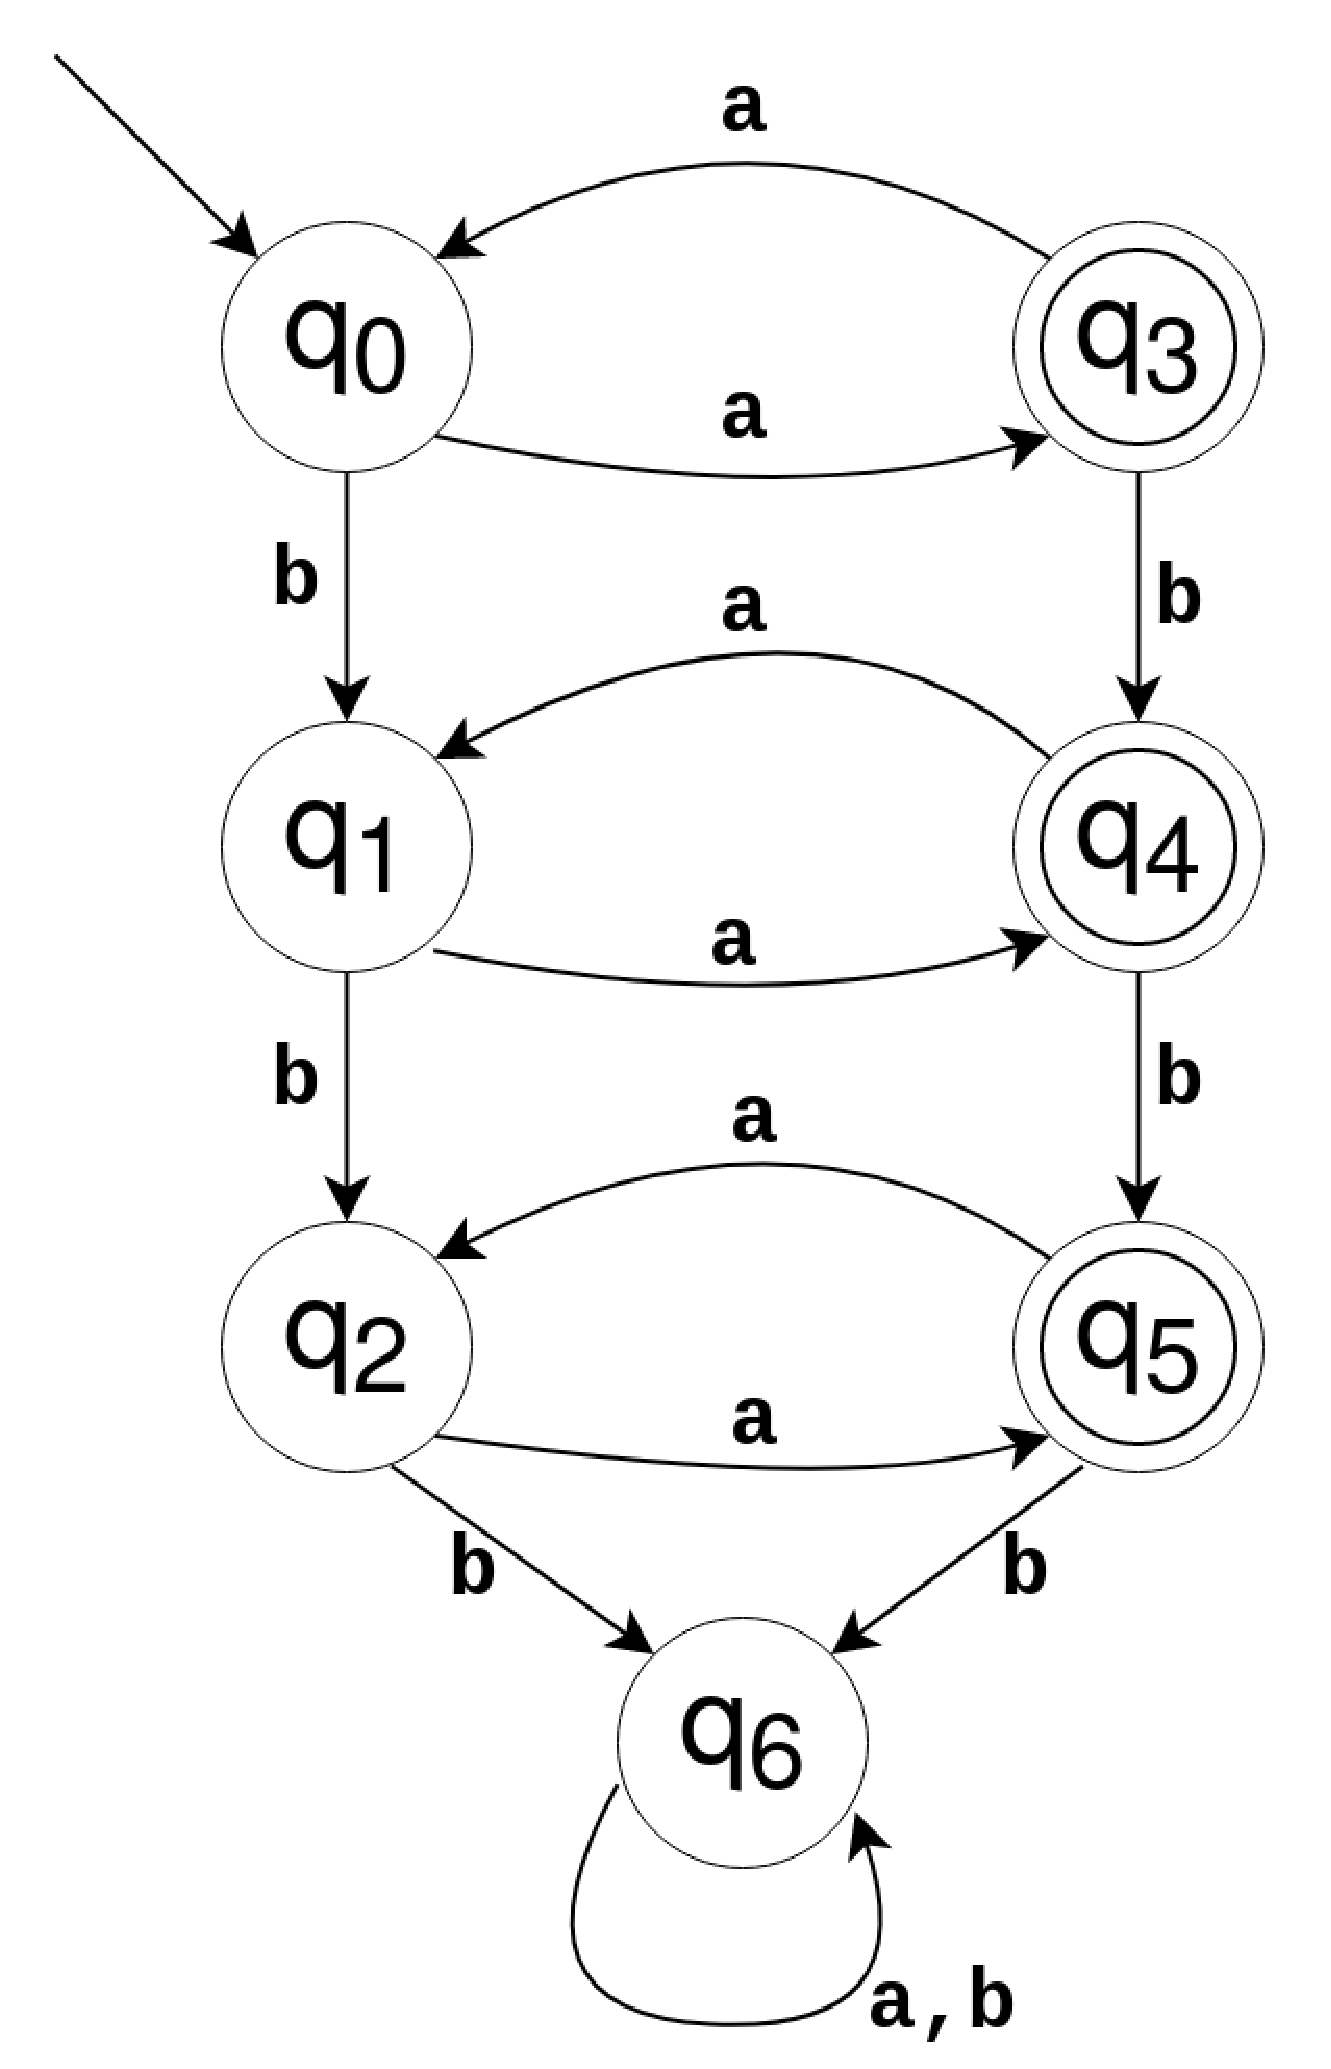
\includegraphics[width=0.5\textwidth]{5.eps}
    \end{center}
    \newpage

    \item Rozklad $\Sigma^* / \sim_L$:

    \begin{equation*}
    \begin{aligned}
        L^{-1}(q_0) = \{w | \#_a(w) mod 2 = 0 \land \#_b(w) = 0 \} \\
        L^{-1}(q_1) = \{w | \#_a(w) mod 2 = 0 \land \#_b(w) = 1 \} \\
        L^{-1}(q_2) = \{w | \#_a(w) mod 2 = 0 \land \#_b(w) = 2 \} \\
        L^{-1}(q_3) = \{w | \#_a(w) mod 2 = 1 \land \#_b(w) = 0 \} \\
        L^{-1}(q_4) = \{w | \#_a(w) mod 2 = 1 \land \#_b(w) = 1 \} \\
        L^{-1}(q_5) = \{w | \#_a(w) mod 2 = 1 \land \#_b(w) = 2 \} \\
        L^{-1}(q_6) = \{w | \#_a(w) mod 2 = 0 \lor  \#_b(w) > 2 \}
    \end{aligned}
    \end{equation*}


\item Relácia $\sim_L$ má konečný index(7), to znamená že jazyk L je regulárny - vyplýva z \textbf{3.21}. Konečný automat, ktorý odpoviedá $\sim_L$ je minimálny konečný automat prijímajúci L.  Zjednotením tried $L^{-1}(q_3), L^{-1}(q_4)$ a $L^{-1}(q_5)$ vznikne jazyk L.

    \begin{equation}
        L = L^{-1}(q_3) \cup L^{-1}(q_4) \cup L^{-1}(q_5) 
    \end{equation}




\end{enumerate}































\newpage
\section{Literatura}
\bibliographystyle{czechiso}
\begin{flushleft}
    \bibliography{quotation}
    \end{flushleft}

\end{document}
